
\section{Application to spectral density approximation}
\label{sec:application}

We now get back to the task of computing the spectral density $1/n \sum_{i=1}^{n} \delta(t - \lambda_i)$ of a real symmetric matrix $\mtx{A} \in \mathbb{R}^{n \times n}$ with eigenvalues $\lambda_1, \dots, \lambda_n$, where $\delta(\cdot)$ denotes the Dirac delta distribution. As explained in the introduction, finding accurate approximations to this distribution is challenging, and we will therefore work with
a smoothed version.

\subsection{Smoothed spectral density}
\label{subsec:spectral-density}

We recall that the smoothed spectral density $\phi_{\sigma}$ is defined as
\begin{equation}
    \phi_{\sigma}(t) = \frac{1}{n} \sum_{i=1}^{n} g_{\sigma}(t - \lambda_i) = \frac{1}{n} \Trace(g_{\sigma}(t\mtx{I}_n - \mtx{A}))
    \label{equ:smooth-spectral-density}
\end{equation}
for a smoothing kernel $g_{\sigma}$ parametrized by a smoothing parameter $\sigma > 0$. In this work, we choose a Gaussian smoothing kernel of width $\sigma > 0$:
\begin{equation}
    g_{\sigma}(s) = \frac{1}{\sigma \sqrt{2\pi}} e^{-\sfrac{s^2}{2\sigma^2}}.
    \label{equ:smoothing-kernel}
\end{equation}
The expression~\refequ{equ:smooth-spectral-density} gives rise to the task of estimating the trace of the parameter-dependent SPSD matrix $g_{\sigma}(t\mtx{I}_n - \mtx{A})$, which has been analyzed in \refsec{sec:analysis}.

Choosing the smoothing parameter $\sigma$ results in the following trade off: A larger $\sigma$ usually makes it  easier to approximate the matrix function $g_{\sigma}(t\mtx{I}_n - \mtx{A})$, whereas a smaller $\sigma$ allow one to stay closer to the original spectral density $\phi$. To quantify the latter, one can measure the error between $\phi$ and its smoothened version $\phi_{\sigma}$ by
\begin{equation}
    \sup_{f \in \mathcal{S}} \int_{a}^{b} f(t) (\phi(t) - \phi_{\sigma}(t))~\mathrm{d}t,
    \label{equ:error-metric}
\end{equation}
where $\mathcal{S}$ represents an appropriately chosen space of test functions. Among others, the reference~\cite{lin-2016-approximating-spectral} uses $\mathcal{S} = \{ f: f(t) \equiv g_{\sigma}(t - s), s \in [a, b]\}$, \cite{chen-2021-analysis-stochastic} uses $\mathcal{S} = \{f : f(t) = \Theta(s - t), s \in [a, b] \}$ with the Heaviside step function $\Theta$, and \cite{braverman-2022-sublinear-time,bhattacharjee-2025-improved-spectral} use $\mathcal{S} = \{f : |f(t) - f(s)| \leq |t - s| \}$ for which the error \refequ{equ:error-metric} is equivalent to the Wasserstein-1 distance between $\phi$ and $\phi_{\sigma}$.
When choosing 
the last metric,
assuming that the eigenvalues are somewhat uniformly distributed and $\sigma$ is rather small, a simple calculation allows one to conclude that the smoothing error \refequ{equ:error-metric} is of the order $\sigma$. Consequently, to ensure that the approximation deviates by at most a factor of $\varepsilon > 0$, one needs to choose $\sigma \approx \varepsilon$.

\subsection{Chebyshev approximation of smoothing kernel}
\label{subsec:chebyshev-approximation}

To estimate the trace in \refequ{equ:smooth-spectral-density} efficiently, we approximate the function 
$s\mapsto g_{\sigma}(t- s)$ by a
Chebyshev approximation $g_{\sigma}^{(m)}(t-s) = 
\sum_{l=0}^{m} \mu_l(t) T_l(s)$
with the approximation coefficients $\mu_l(t) \in \mathbb R$ and the Chebyshev polynomials
$T_l(s) = \cos(l \cdot \arccos(s))$ for $l = 0,1,\ldots,m$. We choose the coefficients $\mu_l(t)$ in such a way that $g_{\sigma}^{(m)}(t-s)$ interpolates $g_{\sigma}(t-s)$ at the Chebyshev nodes $s_i = \cos(\pi i / m),~i=0,1,\dots,m$. In this case, $g_{\sigma}^{(m)}$ is often referred to as the Chebyshev interpolant~\cite[Chapter 2]{trefethen-2020-approximation-theory}.
Assuming that the spectrum of $\mtx{A}$ is contained in $[-1,1]$, this gives rise to
\begin{equation}
    g_{\sigma}(t\mtx{I}_n - \mtx{A}) \approx g_{\sigma}^{(m)}(t\mtx{I}_n - \mtx{A}) = \sum_{l=0}^{m} \mu_l(t) T_l(\mtx{A}).
    \label{equ:matrix-approximation}
\end{equation}
Inserting~\refequ{equ:matrix-approximation} into~\refequ{equ:smooth-spectral-density} yields the approximate smoothed spectral density
\begin{equation}
    \phi_{\sigma}(t) \approx \phi_{\sigma}^{(m)}(t) =  \frac{1}{n} \Trace(g_{\sigma}^{(m)}(t \mtx{I}_n - \mtx{A})).
    \label{equ:expanded-spectral-density}
\end{equation}
\begin{remark}
For a general symmetric matrix $\mtx{A}$, one first estimates an interval $[a,b]$ containing the spectrum of $\mtx{A}$~\cite{zhou-2011-bounding-spectrum}. The usual affine transform
$\tau(t) = \frac{2t - a - b}{b - a}$
then lets us define a matrix $\bar{\mtx{A}} = \tau(\mtx{A})$ for which the spectrum is contained in $[-1, 1]$ and, hence, the approximation \refequ{equ:matrix-approximation} is sensible.\footnote{Note that one has to adjust the smoothing parameter $\bar{\sigma} = 2 \sigma (b - a)^{-1}$ to obtain an undistorted approximation of the original spectrum when inverting the transformation.} This allows to assume, from now on and without loss of generality, that the spectrum of $\mtx{A}$ is contained in $[-1, 1]$.
\end{remark}


\subsubsection{Approximation error}
\label{subsubsec:approximation-error}

We now analyze the impact of the Chebyshev approximation of the Gaussian smoothing kernel $g_{\sigma}$ in the approximation of the spectral density $\phi_{\sigma}$. We start with a standard error estimate concerning the approximation of $g_{\sigma}$.

\begin{lemma}{Chebyshev approximation error}{chebyshev-error}
    The Chebyshev approximation $g_{\sigma}^{(m)}$ of the Gaussian smoothing kernel $g_{{\sigma}}$ from  \refequ{equ:smoothing-kernel} satisfies
    \begin{equation}
        \sup_{s,t \in [-1, 1]} \big| g_{\sigma}(t - s) - g_{\sigma}^{(m)}(t - s) \big| \leq 2\sqrt{\frac{2e}{\pi}} \frac{1}{\sigma^2} (1 + \sigma)^{-m} =: E_{\sigma, m}
        \label{equ:chebyshev-interpolation-sup-error-kernel}
    \end{equation}
    for every degree $m \in \mathbb{N}$ and smoothing parameter $\sigma > 0$.
\end{lemma}
\begin{proof}
    The proof of this result is standard. Let $\mathcal{E}_{\chi} \subset \mathbb{C}$ denote the Bernstein ellipse  with foci $\{-1, +1\}$ and the sum of semi-axes equal to $\chi > 1$. By\cite[Theorem 8.2]{trefethen-2020-approximation-theory},
    \begin{equation*}
        \sup_{s \in [-1, 1]} \big| g_{\sigma}(t - s) - g_{\sigma}^{(m)}(t - s) \big| \leq \frac{4}{\chi^m (\chi - 1)} \max_{z \in \mathcal{E}_{\chi}} |g_{\sigma}(t - z)|,
        \label{equ:bernstein-bound}
    \end{equation*}
    where used the analyticity of $g_{\sigma}(t- \cdot)$.
    For $z = x + \mathrm{i} y \in \mathcal{E}_{\chi}$, we have
    \begin{equation*}
    | g_{\sigma}(t - z) | 
    = \frac{1}{\sigma \sqrt{2 \pi}} \big| e^{-\sfrac{(t - z)^2}{2\sigma^2}} \big|
    = \frac{1}{\sigma \sqrt{2 \pi}} e^{-\sfrac{(t - x)^2}{2\sigma^2}}e^{\sfrac{y^2}{2\sigma^2}}
    \le \frac{1}{\sigma \sqrt{2 \pi}} e^{\sfrac{(\chi - \chi^{-1})^2}{8 \sigma^2}},
    \end{equation*}
    where the last inequality uses 
    $e^{-\sfrac{(t - x)^2}{2\sigma^2}} \leq 1$ and $|y| \le (\chi - \chi^{-1}) / 2$.
    Choosing $\chi = 1 + \sigma$ and using $\chi - \chi^{-1} \leq 2\sigma$ completes the proof of~\refequ{equ:chebyshev-interpolation-sup-error-kernel}.
\end{proof}

A simple algebraic manipulation shows that \reflem{lem:chebyshev-error} implies that choosing a degree $m = \mathcal{O}((\log(\varepsilon^{-1}) + \log(\sigma^{-1})) / \log(1 + \sigma))$ ensures an error $\mathcal{O}(\varepsilon)$. The lemma also allows us to bound the $L^1$-error of the spectral density approximation
$\phi_{\sigma}^{(m)}$ defined in~\refequ{equ:expanded-spectral-density}:
\begin{align}
    \int_{-1}^{1} \left| \phi_{\sigma}(t) - \phi_{\sigma}^{(m)}(t) \right|~\mathrm{d}t 
    &= \int_{-1}^{1} \left| \frac{1}{n} \sum_{i=1}^n \big(g_{\sigma}(t - \lambda_i) - g_{\sigma}^{(m)}(t - \lambda_i)\big) \right|~\mathrm{d}t \notag \\
    &\leq \int_{-1}^{1} \max_{i = 1, \dots, n} \big| g_{\sigma}(t - \lambda_i) - g_{\sigma}^{(m)}(t - \lambda_i) \big|~\mathrm{d}t    \leq 2 E_{\sigma, m}.
    \label{equ:chebyshev-interpolation-spectral-density}
\end{align}

\subsubsection{Preservation of non-negativity} \label{sec:preservnonneg}

In general, the Chebyshev approximation $g_{\sigma}^{(m)}$ does not inherit the  non-negativity of the smoothing kernel $g_{\sigma}$. Consequently, the matrix $g_{\sigma}^{(m)}(t \mtx{I}_n - \mtx{A})$ may become 
(slightly) indefinite. This causes issues when attempting to apply the Nyström++ trace estimator (\refalg{equ:nystrompp-trace-estimator}). While we have never observed this in our numerical experiments, the Nyström approximation may fail when the SPSD condition is not met; see also the discussion in~\cite{nakatsukasa-2023-randomized-lowrank}. On the theoretical side,~\refthm{thm:nystrom-pp}
critically relies on the SPSD condition.

To ensure a non-negative Chebyshev approximation, we suggest the following simple method: Given an even degree $m$, approximate the square root of the smoothing kernel up to degree $m/2$:
\begin{equation}
    \sqrt{g_{\sigma}}(t - s) \approx \sqrt{g_{\sigma}}^{(\sfrac{m}{2})}(t - s) = \sum_{l=0}^{m/2} \xi_l(t) T_l(s).
    \label{equ:square-root-chebyshev-approximation}
\end{equation}
When squaring this approximation, one obtains a polynomial of degree $m$, which admits an exact approximation
of the form 
$(\sum_{l=0}^{m/2} \xi_l(t) T_l(s))^2 = \sum_{l=0}^{m} \underline{\mu}_l(t) T_l(s)$.
Thus, we obtain the non-negative Chebyshev approximation
\begin{equation}
g_{\sigma}(t - s) \approx    \underline{g}_{\sigma}^{(m)}(t - s) = \sum_{l=0}^{m} \underline{\mu}_l(t) T_l(s).
    \label{equ:non-negative-chebyshev-approximation}
\end{equation}
The corresponding non-negative approximation of the smoothed spectral density,
\begin{equation}
    \phi_{\sigma}(t) \approx \underline{\phi}_{\sigma}^{(m)}(t) := \frac{1}{n} \Trace(\underline{g}_{\sigma}^{(m)}(t\mtx{I}_n - \mtx{A})),
    \label{equ:non-negative-expanded-density}
\end{equation}
satisfies the following bound.

\begin{lemma}{$L^1$-error of non-negative approximate smooth spectral density}{non-negative-chebyshev-error}
Let $\phi_{\sigma}$ be the smoothed spectral density defined in~\refequ{equ:smooth-spectral-density}
for a symmetric matrix $\mtx{A} \in \mathbb{R}^{n \times n}$ with spectrum contained in $[-1, 1]$. Then the approximation $\underline{\phi}_{\sigma}^{(m)}$ defined in~\refequ{equ:non-negative-expanded-density} satisfies
    \begin{equation*}
        \int_{-1}^{1} \big| \phi_{\sigma}(t) - \underline{\phi}_{\sigma}^{(m)}(t) \big|~\mathrm{d}t \leq 4 \sqrt{2} \left(1 + \sigma \sqrt{\pi} \cdot E_{\sqrt{2}\sigma, \sfrac{m}{2}}\right) E_{\sqrt{2}\sigma, \sfrac{m}{2}} =: \underline{E}_{\sigma, m}
        \label{equ:chebyshev-interpolation-sup-error-kernel-nonneg}
    \end{equation*}
    for every \emph{even} degree $m \in \mathbb{N}$, smoothing parameter $\sigma > 0$, and with $E_{\sigma, m}$ defined in \reflem{lem:chebyshev-error}.
\end{lemma}
\begin{proof}
    Using that the inequality $| a - b | \leq (2 \sqrt{a} + | \sqrt{a} - \sqrt{b} |)  | \sqrt{a} - \sqrt{b} |$ holds for any non-negative numbers $a, b$, it follows that
    \begin{equation*}
        \big| g_{\sigma} - \underline{g}_{\sigma}^{(m)} \big| \leq \big( 2 \big| \sqrt{g_{\sigma}} \big| + \big| \sqrt{g_{\sigma}} - \sqrt{g_{\sigma}}^{(\sfrac{m}{2})} \big| \big) \big| \sqrt{g_{\sigma}} - \sqrt{g_{\sigma}}^{(\sfrac{m}{2})} \big|.
    \end{equation*}
    Because of $\sqrt{g_{\sigma}} = \sqrt{2 \sigma \sqrt{2 \pi}} \cdot g_{\sqrt{2}\sigma}$,
we can apply \reflem{lem:chebyshev-error} with the substitutions
    $\sigma \gets \sqrt{2}\sigma$ and $m \gets m/2$ to bound 
    $\big| \sqrt{g_{\sigma}} - \sqrt{g_{\sigma}}^{(\sfrac{m}{2})} \big|$.
    Together with  $|\sqrt{g_{\sigma}}| \leq 1/\sqrt{\sigma \sqrt{2 \pi}}$, we get
    \begin{align*}
        \big| g_{\sigma}(t - s) - \underline{g}_{\sigma}^{(m)}(t - s) \big| \notag 
        &\leq \Big( 2 \frac{1}{\sqrt{ \sigma \sqrt{2\pi}}} + \sqrt{2 \sigma \sqrt{2 \pi}} \cdot E_{\sqrt{2}\sigma, \sfrac{m}{2}}\Big)\sqrt{2 \sigma \sqrt{2 \pi}} \cdot E_{\sqrt{2}\sigma, \sfrac{m}{2}} \notag \\
        &= 2\sqrt{2} \big(1 + \sigma \sqrt{\pi} \cdot E_{\sqrt{2}\sigma, \sfrac{m}{2}}\big) E_{\sqrt{2}\sigma, \sfrac{m}{2}}
    \end{align*}
    for every $s,t \in [-1, 1]$.
    Bounding the integral as in~\refequ{equ:chebyshev-interpolation-spectral-density} then yields the desired result.
\end{proof}

Again, \reflem{lem:non-negative-chebyshev-error} implies that choosing a degree $m = \mathcal{O}((\log(\varepsilon^{-1}) + \log(\sigma^{-1})) / \log(1 + \sigma))$ ensures an error $\mathcal{O}(\varepsilon)$.

As the non-negative approximation~\refequ{equ:non-negative-chebyshev-approximation} ``wastes'' half of the degrees of freedom, it can be expected to be less accurate than the standard Chebyshev approximation. On the other hand, $\sqrt{g_{\sigma}} \propto g_{\sqrt{2}\sigma}$ is somewhat easier to approximate because it is less \enquote{pointy} compared to $g_{\sigma}$. Overall, it turns out that one needs to choose the degree of the non-negative approximation roughly a factor $\sqrt{2}$ larger to match the approximation error of the standard Chebyshev approximation (see also \reffig{fig:interpolation-issue}).

\subsubsection{Computation of Chebyshev coefficients}
\label{subsubsec:dct}

It is well known that the coefficients of the Chebyshev approximation \refequ{equ:matrix-approximation} can --- in exact arithmetic --- be computed by inverting the (type I) discrete cosine transform (DCT)
\begin{equation*}
    g_{\sigma}(t - \cos(s_i)) = \sum_{l=0}^{m} \mu_l(t) \cos\left(\frac{\pi i l}{m} \right)
    \label{equ:discrete-cosine-transform}
\end{equation*}
between the approximation coefficients $\mu_l(t),~l=0,\dots,m$ and the function evaluations at the Chebyshev points $s_i = \cos(\pi i / m),~i=0,\dots,m$ \cite{baszenski-1997-fast-polynomial, plonka-2018-numerical-fourier, trefethen-2020-approximation-theory}. This can be accomplished in $\mathcal{O}(m \log(m))$ operations.

A Chebyshev approximation can be squared in $\mathcal{O}(m \log(m))$ operations by using the DCT and its inverse \cite{baszenski-1997-fast-polynomial}; see \refalg{alg:chebyshev-squaring}. This allows one to efficiently compute the non-negative Chebyshev approximation \refequ{equ:non-negative-chebyshev-approximation}, and it will find further use in \refsec{subsec:chebyshev-nystrom}. 

\begin{algo}{Fast squaring of Chebyshev approximations}{chebyshev-squaring}
    \begin{algorithmic}[1]
        \Statex \textbf{Input:} Coefficients $\{ \mu_l \}_{l=0}^{m}$ of Chebyshev approximation $\sum_{l=0}^{m} \mu_l T_l$
        \Statex \textbf{Output:} Coefficients $\{ \nu_l \}_{l=0}^{2m}$ such that $\sum_{l=0}^{2m} \nu_l T_l = (\sum_{l=0}^{m} \mu_l T_l)^2$
        \State By appending $m$ zeros, define vector $\vct{\mu} = [\mu_0, \ldots, \mu_m,0,\ldots,0 ] \in \mathbb{R}^{2m + 1}$.
    \State Compute $\vct{f} = \operatorname{DCT}(\vct{\mu})$
    \State Compute $[\nu_0, \dots, \nu_{2m}] = \operatorname{DCT}^{-1}(\vct{f} \odot \vct{f})$
    \label{lin:inverse-DCT}
    \end{algorithmic}
\end{algo}
On \reflin{lin:inverse-DCT} of \refalg{alg:chebyshev-squaring}, the symbol $\odot$ denotes the entrywise product. 

In \cite{lin-2017-randomized-estimation}, a slightly different approach to approximating $g_{\sigma}$ is taken: Instead of Chebyshev interpolation,
the kernel $g_{\sigma}$ is approximated by a Chebyshev series~\cite[Chapter 4]{trefethen-2020-approximation-theory} truncated after term $m$. In contrast to interpolation, the expansion coefficients involve integrals, which need to be approximated by quadrature. By choosing $2m+1$ Chebyshev quadrature nodes, this approximation can be carried using the fast Fourier transform (FFT). Although interpolation and truncated expansion satisfy nearly identical convergence bounds~\cite[Theorem 8.2]{trefethen-2020-approximation-theory}, we observed the procedure from~\cite{lin-2017-randomized-estimation} to be significantly slower due to need of applying the FFT (instead of DCT) to longer vectors. See~\reftab{tab:chebyshev-timing-interpolation}, where we compare a benevolent implementation of \cite[Algorithm 1]{lin-2017-randomized-estimation} with our approach, both for the standard and the non-negative Chebyshev approximation.%}

\begin{table}[ht]
    \caption{Runtime in milliseconds for computing the coefficients of a degree-$m$ Chebyshev approximation to the smoothing kernel $g_{\sigma}$ in three different ways. \emph{FFT}: Using~\cite[Algorithm 1]{lin-2017-randomized-estimation}.  \emph{DCT}: Applying the discrete cosine transform directly to $g_\sigma$.  \emph{Non-negative DCT}: Applying the discrete cosine transform to $\sqrt{g_\sigma}$ together with \refalg{alg:chebyshev-squaring}. We use $\sigma=0.005$, $n_t=1000$ parameter values, and various degrees $m$. We average over 7 runs of the algorithms and repeat this $1000$ times to form the mean and standard deviation reported below.}
    \label{tab:chebyshev-timing-interpolation}
   \centering
\renewcommand{\arraystretch}{1.2}
\begin{tabular}{@{}lcccc@{}}
\toprule
 & $m=800$ & $m=1600$ & $m=2400$ & $m=3200$\\
\midrule
FFT & $195.1$ $\pm$ $2.8$ & $1219.7$ $\pm$ $4.2$ & $711.0$ $\pm$ $16.5$ & $1149.2$ $\pm$ $6.4$ \\
DCT & $90.2$ $\pm$ $77.8$ & $85.7$ $\pm$ $0.8$ & $113.1$ $\pm$ $0.4$ & $140.0$ $\pm$ $0.4$ \\
non-negative DCT & $147.1$ $\pm$ $0.6$ & $178.8$ $\pm$ $1.3$ & $210.4$ $\pm$ $0.9$ & $238.6$ $\pm$ $0.6$ \\
\bottomrule
\end{tabular}

\end{table}

\subsection{Chebyshev-Nyström++ method for spectral density approximation}
\label{subsec:chebyshev-nystrom}

Combining the results of \refsec{sec:analysis} and \refsec{subsec:chebyshev-approximation}, we apply the Nyström++ estimator $\Nystrpp{\mtx{\Omega}}{\mtx{\Psi}}$ from~\refequ{equ:nystrompp-trace-estimator}
to the non-negative 
Chebyshev approximation, which yields the approximation
\begin{equation}
    \phi_{\sigma}(t) \approx \widetilde{\underline{\phi}}_{\sigma}^{(m)}(t) := \frac{1}{n} \Nystrpp{\mtx{\Omega}}{\mtx{\Psi}}(\mtx{B}(t)), \quad \mtx{B}(t) = \underline{g}_{\sigma}^{(m)}(t \mtx{I}_n - \mtx{A}).
    \label{equ:chebyshev-nystrom-formula}
\end{equation}

\subsubsection{Implementation}
\label{subsubsec:chebyshev-nystrom-implementation}

One usually aims at evaluating~\refequ{equ:chebyshev-nystrom-formula} for many values of $t$. In the following, we explain how this can be done efficiently by exploiting 
the well-known three-term recurrence relation of Chebyshev polynomials:
\begin{equation}
    T_0(s) = 1,\quad  T_1(s) = s,\quad 
    T_l(s) = 2 s T_{l-1}(s) - T_{l-2}(s) \text{ for $l \geq 2$.}
    \label{equ:chebyshev-recurrence}
\end{equation}

We start with the first term in the definition~\refequ{equ:nystrompp-trace-estimator} of $\Nystrpp{\mtx{\Omega}}{\mtx{\Psi}}$, which requires evaluating the trace of the 
Nyström approximation \refequ{equ:nystrom-approximation}:
\begin{equation}
    \frac{1}{n} \Trace \big((\mtx{B}(t) \mtx{\Omega}) (\mtx{\Omega}^{\top} \mtx{B}(t) \mtx{\Omega})^{\dagger} (\mtx{B}(t) \mtx{\Omega})^{\top} \big) =
    \frac{1}{n} \Trace \big((\underbrace{\mtx{\Omega}^{\top} \mtx{B}(t) \mtx{\Omega}}_{=: \mtx{K}_1(t)})^{\dagger} (\underbrace{\mtx{\Omega}^{\top} \mtx{B}(t)^2 \mtx{\Omega}}_{=: \mtx{K}_2(t)}) \big).
    \label{equ:cyclic-property}
\end{equation}
where we used the invariance of the trace under cyclic permutations.
Inserting the Chebyshev approximation  $\mtx{B}(t) = \underline{g}_{\sigma}^{(m)}(t \mtx{I}_n - \mtx{A})$ gives
\begin{equation*}
    \mtx{K}_1(t) = \mtx{\Omega}^{\top} \underline{g}_{\sigma}^{(m)}(t \mtx{I}_n - \mtx{A}) \mtx{\Omega} = \sum_{l=0}^{m} \underline{\mu}_l(t) (\mtx{\Omega}^{\top} T_l(\mtx{A}) \mtx{\Omega}).
\end{equation*}
Observing that $\mtx{\Omega}^{\top} T_l(\mtx{A}) \mtx{\Omega}$ is independent of $t$ allows us to precompute these (small) $n_{\mtx{\Omega}} \times n_{\mtx{\Omega}}$ matrices for $l=0, \dots, m$ using the Chebyshev recurrence \refequ{equ:chebyshev-recurrence}. For each value of $t$, we then only need to sum these matrices (multiplied by the corresponding coefficient $\underline{\mu}_l(t)$).

The squaring of Chebyshev approximations discussed in \refsec{sec:preservnonneg} allows us to express $\mtx{B}(t)^2 = \underline{g}_{\sigma}^{(m)}(t \mtx{I}_n - \mtx{A})^2 = \sum_{l=0}^{2m} \underline{\nu}_l(t) T_l(\mtx{A})$, where the coefficients $\underline{\nu}_l(t)$ can be cheaply computed from $\underline{\mu}_l(t)$ using~\refalg{alg:chebyshev-squaring}. Hence, if we precompute
$\mtx{\Omega}^{\top} T_l(\mtx{A}) \mtx{\Omega}$
also for $l=m+1, \dots, 2m$, this allows us to evaluate $\mtx{K}_2(t)$ cheaply, in an analogous way to $\mtx{K}_1(t)$. Alternatively, \cite{lin-2017-randomized-estimation} proposes to instead approximate the squared smoothing kernel $g_{\sigma}^2$ in a separate ``auxiliary" Chebyshev series truncated after term $2m$. While this direct approximation of $g_{\sigma}^2$ might be more accurate than our squaring approach, it is \emph{inconsistent} in the sense that numerically computing the truncated Chebyshev series of $g_{\sigma}^2$ gives --- in general --- not the same result as squaring the truncated Chebyshev series of $g_{\sigma}$. We have observed that meticulously ensuring consistency between the approximations of $g_{\sigma}$ and $g_{\sigma}^2$ makes a visible difference in terms of accuracy (cf. \reffig{fig:interpolation-issue}). This consistency will also allow us to derive bounds for the estimator \refequ{equ:chebyshev-nystrom-formula}.

\begin{figure}[ht]
    \centering
    \centering
\renewcommand{\arraystretch}{1.2}
\begin{tabular}{@{}lcccc@{}}
\toprule
 & $m=800$ & $m=1600$ & $m=2400$ & $m=3200$\\
\midrule
FFT & $195.1$ $\pm$ $2.8$ & $1219.7$ $\pm$ $4.2$ & $711.0$ $\pm$ $16.5$ & $1149.2$ $\pm$ $6.4$ \\
DCT & $90.2$ $\pm$ $77.8$ & $85.7$ $\pm$ $0.8$ & $113.1$ $\pm$ $0.4$ & $140.0$ $\pm$ $0.4$ \\
non-negative DCT & $147.1$ $\pm$ $0.6$ & $178.8$ $\pm$ $1.3$ & $210.4$ $\pm$ $0.9$ & $238.6$ $\pm$ $0.6$ \\
\bottomrule
\end{tabular}

    \caption{Accuracy when computing the estimate \refequ{equ:cyclic-property} in three different ways. \emph{Inconsistent}: Applying an auxiliary truncated Chebyshev series to $g_{\sigma}^2$, as proposed in~\cite{lin-2017-randomized-estimation}. \emph{Consistent}: Squaring the Chebyshev approximation $g_{\sigma}^{(m)}$ using \refalg{alg:chebyshev-squaring}. \emph{Non-negative consistent}: Squaring the non-negative Chebyshev approximation $\underline{g}_{\sigma}^{(m)}$ with~\refalg{alg:chebyshev-squaring}. As input matrix we use the $100 \times 100$ matrix $\mtx{A}$ coming from a two-dimensional finite difference discretization of the Hamiltonian defined in~\refequ{equ:electronic-hamiltonian} on a $10 \times 10$ grid. We fix $n_{\mtx{\Omega}} = 80$ to make sure the low-rank approximation is accurate, set $\sigma = 0.005$, and compute the $L^1$ error from the approximation of the spectral density at $n_t = 100$ uniformly spaced values of $t$ in the interval $[-1, 1]$.}
    \label{fig:interpolation-issue}
\end{figure}

To treat the second term in the definition~\refequ{equ:nystrompp-trace-estimator} of $\Nystrpp{\mtx{\Omega}}{\mtx{\Psi}}$, we observe that 
\begin{align}
    &\frac{1}{n n_{\mtx{\Psi}}} \Trace \big(\mtx{\Psi}^{\top} (\mtx{B}(t) - (\mtx{B}(t) \mtx{\Omega}) (\mtx{\Omega}^{\top} \mtx{B}(t) \mtx{\Omega})^{\dagger} (\mtx{B}(t) \mtx{\Omega})^{\top}) \mtx{\Psi}^{\top} \big) \notag \\
    &= \frac{1}{n n_{\mtx{\Psi}}} \big( \underbrace{\Trace(\mtx{\Psi}^{\top} \mtx{B}(t)\mtx{\Psi})}_{=: \ell(t)} - \Trace((\underbrace{\mtx{\Psi}^{\top} \mtx{B}(t) \mtx{\Omega}}_{=: \mtx{L}_1(t)^{\top}}) (\underbrace{\mtx{\Omega}^{\top} \mtx{B}(t) \mtx{\Omega}}_{= \mtx{K}_1(t)^{\top}})^{\dagger} (\underbrace{\mtx{\Omega}^{\top} \mtx{B}(t) \mtx{\Psi}^{\top}}_{=: \mtx{L}_1(t)})) \big).
    \label{equ:cyclic-property-hutchinson}
\end{align}
Each of the annotated terms can be evaluated efficiently for many values of $t$, by precomputing quantities using the Chebyshev recurrence 
$\mtx{B}(t) = \underline{g}_{\sigma}^{(m)}(t \mtx{I}_n - \mtx{A})$, as explained above.

\refalg{alg:nystrom-chebyshev-pp} summarizes the considerations of this section.

\begin{algo}{Chebyshev-Nyström++ method}{nystrom-chebyshev-pp}
\begin{algorithmic}[1]
    \Statex \textbf{Input:} Symmetric $\mtx{A} \in \mathbb{R}^{n \times n}$ with spectrum in $[-1, 1]$, points $\{t_i\}_{i=1}^{n_t} \subset \mathbb{R}$
    \Statex \textbf{Parameters:} Even approximation degree $m \in \mathbb{N}$, number of Girard-Hutchinson queries $n_{\mtx{\Psi}} \in \mathbb{N}_0$, Nyström sketch size $n_{\mtx{\Omega}} \in \mathbb{N}_0$,  smoothing parameter $\sigma > 0$
    \Statex \textbf{Output:} Spectral density approximation $\{\widetilde{\underline{\phi}}_{\sigma}^{(m)}(t_i)\}_{i=1}^{n_t}$
    \For {$i = 1, \dots, n_t$}
        \State Compute coefficients $\{\xi_l(t_i)\}_{l=0}^{\sfrac{m}{2}}$ of Chebyshev approx.~\refequ{equ:square-root-chebyshev-approximation} to $\sqrt{g_{\sigma}}$ with DCT
        \State Compute coefficients $\{\underline{\mu}_l(t_i)\}_{l=0}^{m}$ of non-negative Chebyshev approx. to $g_{\sigma}$ by applying \refalg{alg:chebyshev-squaring} to $\{\xi_l(t_i)\}_{l=0}^{\sfrac{m}{2}}$
        \State Compute coefficients $\{\underline{\nu}_l(t_i)\}_{l=0}^{2m}$ of squared non-negative Chebyshev approx. by applying \refalg{alg:chebyshev-squaring} to $\{\underline{\mu}_l(t_i)\}_{l=0}^{m}$
    \EndFor
    \State Generate Gaussian random matrices $\mtx{\Omega} \in \mathbb{R}^{n \times n_{\mtx{\Omega}}}$, $\mtx{\Psi} \in \mathbb{R}^{n \times n_{\mtx{\Psi}}}$
    \State Initialize $[\mtx{V}_1, \mtx{V}_2, \mtx{V}_3] \gets [\mtx{0}_{n \times n_{\mtx{\Omega}}}, \mtx{\mtx{\Omega}}, \mtx{0}_{n \times n_{\mtx{\Omega}}}]$
    \State Initialize $[\mtx{W}_1, \mtx{W}_2, \mtx{W}_3] \gets [\mtx{0}_{n \times n_{\mtx{\Psi}}}, \mtx{\Psi}, \mtx{0}_{n \times n_{\mtx{\Psi}}}]$
    \State Initialize $[\mtx{K}_1(t_i), \mtx{K}_2(t_i)] \gets [\mtx{0}_{n_{\mtx{\Omega}} \times n_{\mtx{\Omega}}}, \mtx{0}_{n_{\mtx{\Omega}} \times n_{\mtx{\Omega}}}]$ for all $t_i$
    \State Initialize $[\mtx{L}_1(t_i), \ell(t_i)] \gets [\mtx{0}_{n_{\mtx{\Omega}} \times n_{\mtx{\Psi}}}, 0]$ for all $t_i$
    \For {$l = 0, \dots, 2m$}
    \State $[\mtx{X}, \mtx{Y}] \gets \mtx{\mtx{\Omega}}^{\top} [\mtx{V}_2, \mtx{W}_2]$  
      \State $z \gets \Trace(\mtx{\Psi}^{\top} \mtx{W}_2)$
      \For {$i = 1, \dots, n_t$}
        \If {$l \leq m$}
            \State $\mtx{K}_1(t_i) \gets \mtx{K}_1(t_i) + \underline{\mu}_l(t_i) \mtx{X}$ \Comment{assembles $\mtx{\Omega}^{\top} \underline{g}_{\sigma}^{(m)}(t\mtx{I}_n - \mtx{A}) \mtx{\Omega}$}
            \State $\mtx{L}_1(t_i) \gets \mtx{L}_1(t_i) + \underline{\mu}_l(t_i) \mtx{Y}$ \Comment{assembles $\mtx{\Omega}^{\top} \underline{g}_{\sigma}^{(m)}(t\mtx{I}_n - \mtx{A}) \mtx{\Psi}$}
            \State $\ell(t_i) \gets \ell(t_i) + \underline{\mu}_l(t_i) z$ \Comment{assembles $\Trace(\mtx{\Psi}^{\top} \underline{g}_{\sigma}^{(m)}(t\mtx{I}_n - \mtx{A}) \mtx{\Psi})$}
        \EndIf
        \State $\mtx{K}_2(t_i) \gets \mtx{K}_2(t_i) + \underline{\nu}_l(t_i) \mtx{X}$ \Comment{assembles $\mtx{\Omega}^{\top} \underline{g}_{\sigma}^{(m)}(t\mtx{I}_n - \mtx{A})^2 \mtx{\Omega}$}
      \EndFor
      \State $[\mtx{V}_3, \mtx{W}_3] \gets (2 - \delta_{l0}) \mtx{A} [\mtx{V}_2, \mtx{W}_2] - [\mtx{V}_1, \mtx{W}_1]$ \Comment{Chebyshev recurrence}
      \State $[\mtx{V}_1, \mtx{W}_1] \gets [\mtx{V}_2, \mtx{W}_2]$
      \State $[\mtx{V}_2, \mtx{W}_2] \gets [\mtx{V}_3, \mtx{W}_3]$
    \EndFor
    \For {$i = 1, \dots, n_t$}
      \State $\widetilde{\underline{\phi}}_{\sigma}(t_i) \gets \frac{1}{n} \Trace\left( \mtx{K}_1(t_i)^{\dagger}\mtx{K}_2(t_i) \right) + \frac{1}{n n_{\mtx{\Psi}}} \left( \ell(t_i) + \Trace\left( \mtx{L}_1(t_i)^{\top} \mtx{K}_1(t_i)^{\dagger} \mtx{L}_1(t_i) \right)  \right) $ \label{lin:4-nystromchebyshev-nystrom-pp}
    \EndFor
\end{algorithmic}
\end{algo}

\refalg{alg:nystrom-chebyshev-pp} requires $(2m + 1)(n_{\mtx{\Psi}} + n_{\mtx{\Omega}})$ matrix-vector multiplications with $\mtx{A}$, which can be expected to dominate its cost. For each of the evaluation points $t_1, \dots, t_{n_t}$ another $\mathcal{O}(m \log(m) + m (n_{\mtx{\Omega}}^2 + n_{\mtx{\Omega}} n_{\mtx{\Psi}} + 1) + (n_{\mtx{\Omega}}^3 + n_{\mtx{\Omega}} n_{\mtx{\Psi}}^2 + 1))$ operations are needed, which is independent of $n$ --- thanks to the precomputations discussed above.

\refalg{alg:nystrom-chebyshev-pp} also accommodates the other two estimators discussed in \refsec{sec:analysis}: For $n_{\mtx{\Omega}} = 0$ we recover the Girard-Hutchinson estimator~\refequ{equ:hutchinson-trace-estimator}. For $n_{\mtx{\Psi}} = 0$ we recover the Nyström estimator~\refequ{equ:nystrom-trace-estimator}, provided that $0/0$ is evaluated to $0$ in the second term on \reflin{lin:4-nystromchebyshev-nystrom-pp}. In this case, \refalg{alg:nystrom-chebyshev-pp} essentially amounts to the \enquote{spectrum sweeping} method from \cite[Algorithm 5]{lin-2017-randomized-estimation}, featuring a significantly lower computational complexity.

The two pseudoinverses on \reflin{lin:4-nystromchebyshev-nystrom-pp} need to be computed with care. One way to ensure numerical stability is to 
consider an associated eigenvalue problem and threshold the smallest eigenvalues~\cite{lin-2017-randomized-estimation, epperly-2022-theory-quantum}. However, this makes the algorithm significantly more complicated, and we found that it improves accuracy only slightly. Instead, we use the standard NumPy least-squares solver when applying $\mtx{K}_1(t_i)^{\dagger}$, which is based on the LAPACK DGELSD routine, and likewise truncates the smallest eigenvalues by treating them as zero if they are smaller than a certain threshold. We have found a threshold of $10^{-5}$ times the largest eigenvalue to give the best results in our numerical experiments. 

To ensure numerical accuracy, we found it crucial to separately treat regions
where the spectral density nearly vanishes, because there are no eigenvalues in or close to the region.
Especially for small smoothing parameters $\sigma$, the rapid decay of the Gaussian $g_{\sigma}$ will cause $\mtx{K}_1(t) \approx \mtx{\Omega}^{\top} g_{\sigma}(t\mtx{I}_n - \mtx{A}) \mtx{\Omega}$ to be close to zero for parameter values $t$ located in such regions. Hence, on \reflin{lin:4-nystromchebyshev-nystrom-pp} we would compute the pseudoinverse of an almost zero matrix, which can be extremely unstable; see \reffig{fig:zerocheck}. To detect this situation, we can cheaply compute the Girard-Hutchinson 
estimate $\Trace(\mtx{K}_1(t)) / n_{\mtx{\Omega}}$ of the nuclear norm. If this estimate is small (in our experiments, smaller than $10^{-5}$), we use it as an indicator that $t$ is within a region with a nearly vanishing spectral density, and therefore set $\widetilde{\underline{\phi}}_{\sigma}^{(m)}(t) = 0$ instead of computing the full expression on \reflin{lin:4-nystromchebyshev-nystrom-pp}.

\begin{figure}[ht]
    \centering
    \input{plots/zerocheck.pgf}
    \caption{The difference the non-zero check can make when approximating a spectral density using \refalg{alg:nystrom-chebyshev-pp}. As input matrix we use the $1000 \times 1000$ matrix $\mtx{A}$ coming from a three-dimensional finite difference discretization of the Hamiltonian defined in~\refequ{equ:electronic-hamiltonian} on a $10 \times 10$ grid. We ran the Chebyshev-Nyström++ method with and without estimating if the matrix function is zero before taking its pseudo-inverse. We let $m=2000$, $n_{\mtx{\Omega}}=80$, $n_{\mtx{\Psi}}=0$, and $\sigma = 0.004$. We compute the $L^1$ error from the approximation of the spectral density at $n_t = 100$ uniformly spaced values of $t$ in the interval $[-1, 1]$.}
    \label{fig:zerocheck}
\end{figure}

\color{black}

\subsubsection{Analysis}
\label{subsubsec:chebyshev-nystrom-analysis}

In this section, we analyze the accuracy of Chebyshev-Nyström++ estimate returned by~\refalg{alg:nystrom-chebyshev-pp}. 
\begin{theorem}{Error of Chebyshev-Nyström++ estimate for smoothed spectral density}{chebyshev-nystrom}
    For a smoothing parameter $\sigma > 0$, let $\phi_{\sigma}$ be the smoothed spectral density~\refequ{equ:smooth-spectral-density} of a symmetric matrix $\mtx{A} \in \mathbb{R}^{n \times n}$ with spectrum contained in $[-1, 1]$. Consider $\varepsilon \in (0, 3)$ and $\delta \in (0, 2 e^{-1})$.
    Then the Chebyshev-Nyström++ estimate $\widetilde{\underline{\phi}}_{\sigma}^{(m)}$ 
    satisfies the error bound
    \begin{equation*}
        \int_{-1}^{1} \left| \phi_{\sigma}(t) - \widetilde{\underline{\phi}}_{\sigma}^{(m)}(t) \right|~\mathrm{d}t \leq \varepsilon
        \label{equ:chebyshev-nystrom-error}
    \end{equation*}
    with probability at least $1 - \delta$ for $m = \mathcal{O}((\log(\varepsilon^{-1}) + \log(\sigma^{-1})) / \log(\sigma + 1))$  and $n_{\mtx{\Omega}} = n_{\mtx{\Psi}} = \mathcal{O}(\varepsilon^{-1}\log(\delta^{-1}))$.
\end{theorem}

\begin{proof}
Combining results derived above, we obtain that 
    \begin{align*}
        &\int_{-1}^{1} \left| \phi_{\sigma}(t) - \widetilde{\underline{\phi}}_{\sigma}^{(m)}(t) \right|~\mathrm{d}t \notag \\
        &\leq \int_{-1}^{1} \left| \phi_{\sigma}(t) - \underline{\phi}_{\sigma}^{(m)}(t) \right|~\mathrm{d}t + \int_{-1}^{1} \left| \underline{\phi}_{\sigma}^{(m)}(t) - \widetilde{\underline{\phi}}_{\sigma}^{(m)}(t) \right|~\mathrm{d}t &&  \notag \\
        &\leq \int_{-1}^{1} \left| \phi_{\sigma}(t) - \underline{\phi}_{\sigma}^{(m)}(t) \right|~\mathrm{d}t + \widetilde{\varepsilon} \int_{-1}^{1} \left| \underline{\phi}_{\sigma}^{(m)}(t) \right|~\mathrm{d}t && \text{(\refthm{thm:nystrom-pp} w.p. $\geq 1 - \delta$)} \notag \\
        &\leq (1 + \widetilde{\varepsilon}) \int_{-1}^{1} \left| \phi_{\sigma}(t) - \underline{\phi}_{\sigma}^{(m)}(t) \right|~\mathrm{d}t + \widetilde{\varepsilon} \int_{-1}^{1} \left| \phi_{\sigma}(t) \right|~\mathrm{d}t &&  \notag \\
        &\leq (1 + \widetilde{\varepsilon}) \underline{E}_{\sigma, m} + \widetilde{\varepsilon}. && \text{(\reflem{lem:non-negative-chebyshev-error})} \notag 
    \end{align*}
    From \reflem{lem:non-negative-chebyshev-error} and the discussion after \reflem{lem:chebyshev-error} we see that the choice $m = \mathcal{O}((\log(\widetilde{\varepsilon}^{-1}) + \log(\sigma^{-1})) / \log(\sigma + 1))$ ensures $\underline{E}_{\sigma, m} \leq \widetilde{\varepsilon}$, and thus
    the result follows by setting $\varepsilon = 3 \widetilde{\varepsilon}$.
\end{proof}

In practice, the $\mathcal{O}(\varepsilon^{-1})$ complexity of $n_{\mtx{\Omega}}$ and $n_{\mtx{\Psi}}$ in \refthm{thm:chebyshev-nystrom} is often pessimistic, because  the underlying result of \refthm{thm:nystrom-pp} is agnostic to the low-rank structure of the matrix $\mtx{B}(t) = g_{\sigma}(t\mtx{I}_n - \mtx{A})$. The singular values of this matrix are given by
\begin{equation*}
    \sigma_i(t) = g_{\sigma}(t - \lambda_{(i)}) = \frac{1}{\sigma\sqrt{2 \pi}} \exp\Big( -\frac{(t - \lambda_{(i)})^2}{2 \sigma^2} \Big),  
    \label{equ:gaussian-kernel-eigenvalues}
\end{equation*}
where $\lambda_{(1)}, \dots, \lambda_{(n)}$ denote the eigenvalues of $\mtx{A}$ sorted by increasing distance from $t$, such that $\sigma_1(t) \geq \dots \geq \sigma_n(t) \ge 0$. An eigenvalue $\lambda_{(i)}$ distant from $t$ results in an exponentially small singular value $\sigma_i(t)$. In particular, for a small value of $\sigma$, all singular values corresponding to eigenvalues outside a certain window $[t - d, t + d]$ are negligibly small; see \reffig{fig:numerical-rank}.
\begin{figure}[ht]
    \centering
    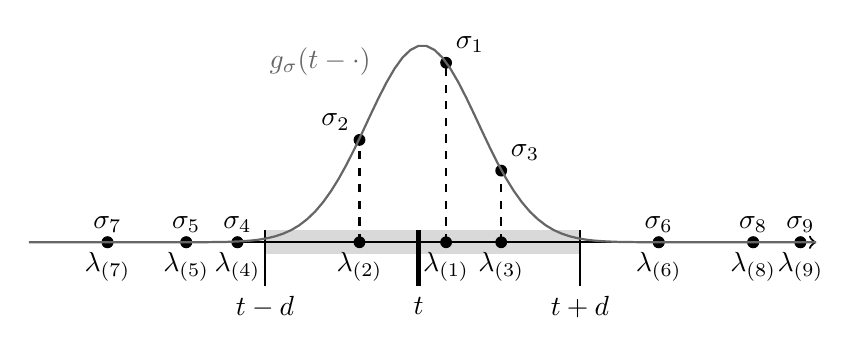
\begin{tikzpicture}
    \fill[black!15!white] (-2.0, -0.15) rectangle (2.0, 0.15);
    \draw[thick, ->] (-5, 0) to (5, 0);
    \fill[black] (-4, 0) circle (0.075) node[below] {$\lambda_{(7)}$};
    \fill[black] (-3, 0) circle (0.075) node[below] {$\lambda_{(5)}$};
    \fill[black] (-2.35, 0) circle (0.075) node[below] {$\lambda_{(4)}$};
    \fill[black] (-0.8, 0) circle (0.075) node[below] {$\lambda_{(2)}$};
    \fill[black] (0.3, 0) circle (0.075) node[below] {$\lambda_{(1)}$};
    \fill[black] (1, 0) circle (0.075) node[below] {$\lambda_{(3)}$};
    \fill[black] (3, 0) circle (0.075) node[below] {$\lambda_{(6)}$};
    \fill[black] (4.2, 0) circle (0.075) node[below] {$\lambda_{(8)}$};
    \fill[black] (4.8, 0) circle (0.075) node[below] {$\lambda_{(9)}$};
    \fill[black] (-4, 0) circle (0.075) node[above] {$\sigma_{7}$};
    \fill[black] (-3, 0) circle (0.075) node[above] {$\sigma_{5}$};
    \fill[black] (-2.35, 0) circle (0.075) node[above] {$\sigma_{4}$};
    \fill[black] (-0.8, 1.3) circle (0.075) node[above left] {$\sigma_{2}$};
    \fill[black] (0.3, 2.28) circle (0.075) node[above right] {$\sigma_{1}$};
    \fill[black] (1, 0.91) circle (0.075) node[above right] {$\sigma_{3}$};
    \fill[black] (3, 0) circle (0.075) node[above] {$\sigma_{6}$};
    \fill[black] (4.2, 0) circle (0.075) node[above] {$\sigma_{8}$};
    \fill[black] (4.8, 0) circle (0.075) node[above] {$\sigma_{9}$};
    \draw[black, ultra thick] (-0.05, 0.15) to (-0.05, -0.55) node[below] {$t$};
    \draw[black, thick] (-2.0, 0.15) to (-2.0, -0.55) node[below] {$t - d$};
    \draw[black, thick] (2.0, 0.15) to (2.0, -0.55) node[below] {$t + d$};
    \draw[black, thick, dashed] (-0.8, 0) to (-0.8, 1.3);
    \draw[black, thick, dashed] (0.3, 0) to (0.3, 2.28);
    \draw[black, thick, dashed] (1, 0) to (1, 0.91);
    \draw[black!60!white, thick] (-5.000, 0.000) to (-4.899, 0.000) to (-4.798, 0.000) to (-4.697, 0.000) to (-4.596, 0.000) to (-4.495, 0.000) to (-4.394, 0.000) to (-4.293, 0.000) to (-4.192, 0.000) to (-4.091, 0.000) to (-3.990, 0.000) to (-3.889, 0.000) to (-3.788, 0.000) to (-3.687, 0.000) to (-3.586, 0.000) to (-3.485, 0.000) to (-3.384, 0.000) to (-3.283, 0.000) to (-3.182, 0.000) to (-3.081, 0.000) to (-2.980, 0.000) to (-2.879, 0.001) to (-2.778, 0.001) to (-2.677, 0.002) to (-2.576, 0.003) to (-2.475, 0.005) to (-2.374, 0.009) to (-2.273, 0.014) to (-2.172, 0.022) to (-2.071, 0.034) to (-1.970, 0.052) to (-1.869, 0.076) to (-1.768, 0.110) to (-1.667, 0.155) to (-1.566, 0.215) to (-1.465, 0.293) to (-1.364, 0.389) to (-1.263, 0.508) to (-1.162, 0.649) to (-1.061, 0.812) to (-0.960, 0.995) to (-0.859, 1.196) to (-0.758, 1.408) to (-0.657, 1.625) to (-0.556, 1.836) to (-0.455, 2.033) to (-0.354, 2.206) to (-0.253, 2.346) to (-0.152, 2.443) to (-0.051, 2.494) to (0.051, 2.494) to (0.152, 2.443) to (0.253, 2.346) to (0.354, 2.206) to (0.455, 2.033) to (0.556, 1.836) to (0.657, 1.625) to (0.758, 1.408) to (0.859, 1.196) to (0.960, 0.995) to (1.061, 0.812) to (1.162, 0.649) to (1.263, 0.508) to (1.364, 0.389) to (1.465, 0.293) to (1.566, 0.215) to (1.667, 0.155) to (1.768, 0.110) to (1.869, 0.076) to (1.970, 0.052) to (2.071, 0.034) to (2.172, 0.022) to (2.273, 0.014) to (2.374, 0.009) to (2.475, 0.005) to (2.576, 0.003) to (2.677, 0.002) to (2.778, 0.001) to (2.879, 0.001) to (2.980, 0.000) to (3.081, 0.000) to (3.182, 0.000) to (3.283, 0.000) to (3.384, 0.000) to (3.485, 0.000) to (3.586, 0.000) to (3.687, 0.000) to (3.788, 0.000) to (3.889, 0.000) to (3.990, 0.000) to (4.091, 0.000) to (4.192, 0.000) to (4.293, 0.000) to (4.394, 0.000) to (4.495, 0.000) to (4.596, 0.000) to (4.697, 0.000) to (4.798, 0.000) to (4.899, 0.000) to (5.000, 0.000);
    \node[black!60!white] at (-1.3, 2.3) {$g_{\sigma}(t - \cdot)$};
\end{tikzpicture}

    \caption{Singular values $\sigma_i$ of $g_{\sigma}(t\mtx{I}_n - \mtx{A})$ corresponding to eigenvalues $\lambda_{(i)}$ of $\mtx{A}$ which lie further away from $t$ than a certain distance $d$ are negligibly small.}
    \label{fig:numerical-rank}
\end{figure}
By choosing $n_{\mtx{\Omega}}$ such that the sum $\sum_{i=n_{\mtx{\Omega}}+5}^{n} \sigma_i(t)$ becomes negligibly small,  \refthm{thm:nystrom} implies an excellent approximation with high probability. In particular, if we assume the eigenvalues of $\mtx{A}$ to be roughly uniformly distributed, a small calculation shows that $n_{\mtx{\Omega}} = \mathcal{O}(n \sigma \sqrt{\log(\varepsilon^{-1}) + \log(\sigma^{-1})})$ will ensure this.
